%-*- ES -*-
%----------------------------------------------------------------------
% Capitulo 7: Descripción del problema

En éste capítulo se verá por qué los protocolos http y smtp son inseguros, introducción al snnifin, spoofing, arp attack
%----------------------------------------------------------------------

(Agregar una intro)


\section{Riesgos de intermediarios}

Un intermediario es alguien que puede ver el contenido de lo que circula por 
la red. A esta actividad o ataque se lo conoce como “man-in-the-middle” u 
hombre en el medio. Los intermediarios pueden tener acceso a información 
relacionada con la seguridad, información personal sobre usuarios individuales 
y organizaciones, o contenido propietario de usuarios y proveedores de 
contenido. HTTP en sí mismo no puede resolver este problema.

En este proyecto, explotaremos esta vulnerabilidad para demostrar la facilidad
 con la que un agente puede hacerse de nuestro tráfico.


\section{(posible a irse) Ataques a traves de la longitud del elemento del protocolo}

Debido a que HTTP utiliza principalmente campos textiales delimitados por caracteres,
los analizadores a menudo son vulnerables a ataques basados en el envío de 
flujos de datos muy largos (o muy lentos), particularmente cuando una 
implementación espera un elemento de protocolo sin una longitud predefinida.


\section{División de respuesta}


La división de respuestas aprovecha una vulnerabilidad en los servidores 
(generalmente dentro de un servidor de aplicaciones) donde un atacante 
puede enviar datos codificados dentro de algún parámetro de la solicitud 
que luego se decodifica y se repite dentro de cualquiera de los campos de 
encabezado en la respuesta. Si los datos decodificados están diseñados para 
que parezca que la respuesta ha finalizado y ha comenzado una respuesta 
posterior, la respuesta se ha dividido y el atacante controla el contenido 
de la segunda respuesta aparente. Luego, el atacante puede realizar 
cualquier otra solicitud en la misma conexión persistente y engañar a los 
destinatarios (incluidos los intermediarios) para que crean que la segunda 
mitad de la división es una respuesta autorizada a la segunda solicitud.



\section{Integridad de los mensajes}

HTTP no define un mecanismo específico para garantizar la integridad de los 
mensajes, sino que se basa en la capacidad de detección de errores de los 
protocolos de transporte subyacentes y en el uso de tramas delimitadas por 
longitud. Históricamente, la falta de un mecanismo de integridad único se 
ha justificado por la naturaleza informal de la mayoría de las comunicaciones 
HTTP. Sin embargo, el predominio de HTTP como mecanismo de acceso a la 
información ha dado como resultado la necesidad de veririficar la integridad
en ciertos entornos.

\section{Confidencialidad del mensaje}

De la misma manera que en la integridad del mensaje, HTTP se basa en 
protocolos de transporte subyacentes para brindar confidencialidad a los 
mensajes cuando se desee. Por sí solo, el protocolo no cifra los mensajes, 
sin embargo, dado que HTTP se ha diseñado para ser independiente del protocolo de 
transporte, de modo que se puede utilizar en muchas formas diferentes de 
conexión cifrada.


\section{Tipos de ataques}
Existen principalmente dos tipos de ataques a la red: ataques pasivos y 
ataques activos. La motivación detrás de los atacantes pasivos y los atacantes 
activos son totalmente diferentes. Mientras que la motivación de los atacantes 
pasivos es simplemente robar información sensible y analizar el tráfico para 
robar mensajes futuros, la motivación de los atacantes activos es detener la 
comunicación normal entre dos entidades legítimas.

\subsection{Passive Attacks}
Los ataques pasivos ocurren cuando se monitorea y analiza 
información sensible, posiblemente comprometiendo la seguridad de las 
empresas y sus clientes. 

Los atacantes pasivos están principalmente interesados en robar información 
confidencial. Esto sucede sin el conocimiento de la víctima. Como tales, 
los ataques pasivos son difíciles de detectar y, por lo tanto, es dificil de
proteger la red de los mismos. Entre los ataques mas comunes estan los 
ataques de análisis y monitoreo de tráfico, como así también las 
escuchas de comunicaciones telefónicas.

\subsection{Active Attacks}
Los ataques activos ocurren cuando la información se modifica, se altera o 
se destruye por completo. Aquí el intruso inicia instrucciones para 
perturbar la comunicación regular de la red. Algunos de los ataques 
activos son los  siguientes:
\begin{itemize}
    \setlength\itemsep{-0.6em}
    \item Modificación: el nodo malicioso realiza algunas alteraciones en la 
    enrutación. Esto da como resultado que el remitente envíe mensajes a 
    través de la ruta larga, lo que provoca un retraso en la comunicación. 
    Este es un ataque a la integridad.
    \item Wormhole(Agujero de gusano): este ataque también se denomina ataque 
    de túnel. Un atacante recibe un paquete en un punto. Luego lo envia 
    a otro nodo malicioso en la red. Esto hace que se piense que se encontró 
    un camino más corto en la red.
    \item Fabricación: un nodo malicioso genera un mensaje de enrutamiento 
    falso que provoca la generación de información incorrecta sobre la ruta 
    entre dispositivos. Este es un ataque a la autenticidad.
    \item Spoofing: un nodo malicioso presenta incorrectamente su identidad 
    para que el remitente cambie su topología, y por consiguiente el 
    destino de sus mensajes.
    \item Denegación de servicios: un nodo malicioso envía un mensaje al 
    nodo y consume el ancho de banda de la red en cómputo desperdiciado.
    \item Ataque Man-in-the-middle: también llamado ataque de secuestro, 
    es un ataque en el que el atacante altera y transmite en secreto 
    las comunicaciones entre dos partes legítimas sin su conocimiento. 
    Estas partes, a su vez, desconocen lo que sucede, pues no perciben 
    un cambio en la comunicación.
\end{itemize}


\section{Caso de estudio: Interceptando la red para obtener credenciales}

\subsection{Herramienta Utilizadas} 
    

\subsubsection*{Kali Linux}
Kali Linux es una distribución de Linux (basada en Debian) centrada en la seguridad. 
Es una versión renombrada de la famosa distribución de Linux conocida como Backtrack, 
que venía con un enorme repositorio de herramientas de piratería de código abierto, 
para pruebas de penetración de aplicaciones \emph{web}, inalámbricas y de red. 

\begin{center}
    \begin{figure}   
       \begin{center}
          
\includegraphics[width=11cm,height=7cm]{ataque-1.png}
       \end{center}
       \caption{Escritorio de Kali Linux}
    \end{figure}
 \end{center}
 

Kali Linux contiene muchas herramientas preinstaladas con 
todas las dependencias y ya está lista para usar. Esto nos permite tener que prestar 
más atención a las pruebas y no a la instalación de la herramienta. Las actualizaciones 
para las herramientas instaladas en Kali Linux se publican con mayor frecuencia, 
lo que le ayuda a mantener las a las mismas actualizadas.

Esta distribución contiene las herramientas necesarias para realizar nuestro
ataque.

\subsubsection*{Wireshark}
Wireshark es uno de los analizadores de protocolos de red más populares, es de 
código abierto y gratuito. Wireshark está preinstalado en Kali y es ideal para la 
resolución de problemas de red, análisis y, para este caso de estudio, una herramienta 
perfecta para monitorear el tráfico de posibles objetivos. Wireshark usa un kit de 
herramientas para implementar su interfaz de usuario y para capturar paquetes. 
Funciona de manera muy similar a un comando \emph{tcpdump}; sin embargo, nos brinda
una interfaz gráfica, posee opciones integradas de clasificación y filtrado.

\begin{center}
    \begin{figure}   
       \begin{center}
          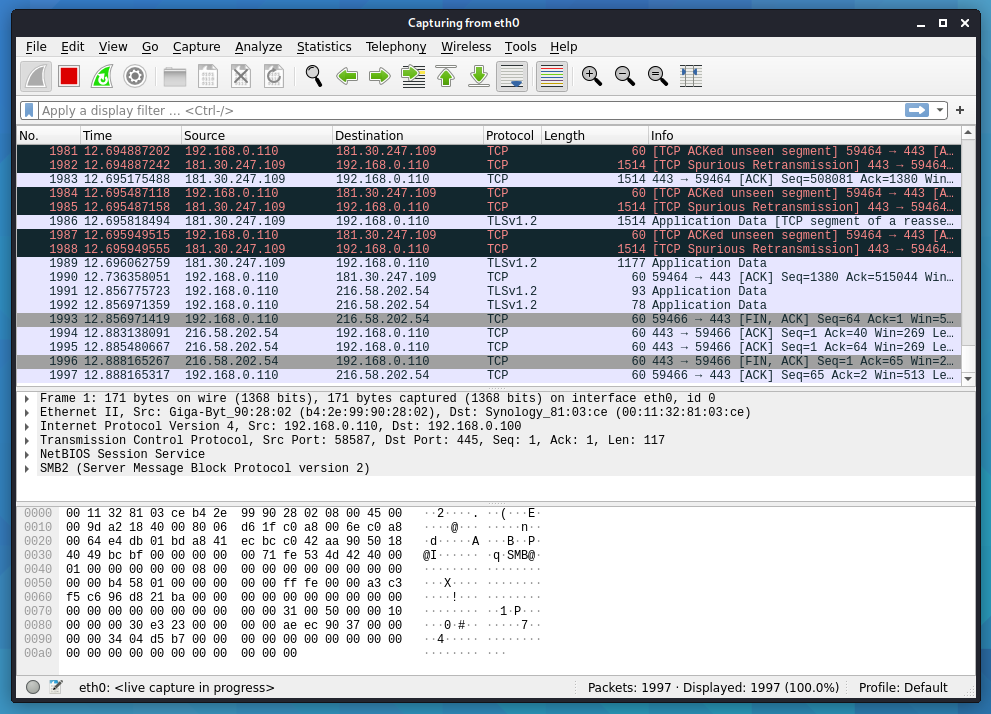
\includegraphics[width=10cm,height=7cm]{wireshark.png}
       \end{center}
       \caption{Interface del Wireshark}
    \end{figure}
 \end{center}
 
\subsubsection*{Ettercap}

\begin{center}
   \begin{figure}   
      \begin{center}
         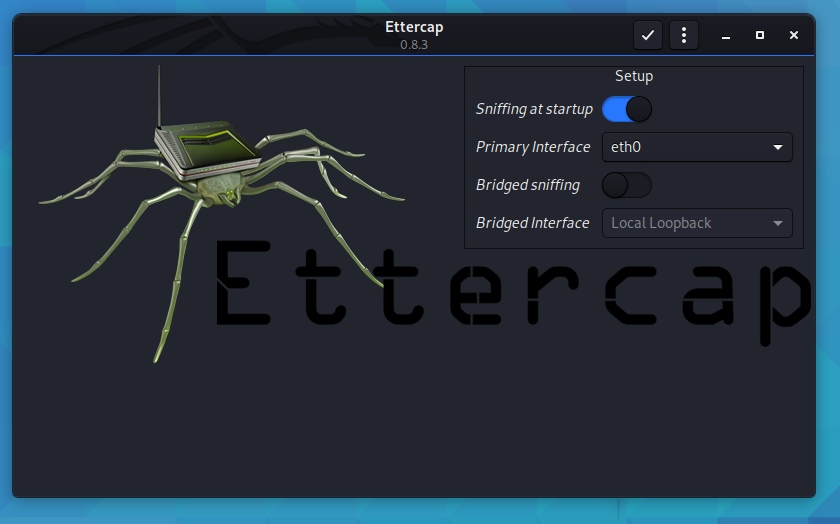
\includegraphics[width=10 cm,height=7cm]{ataque-2.png}
      \end{center}
      \caption{Ettercap}
   \end{figure}
\end{center}

Ettercap es un paquete completo gratuito y de código abierto para ataques basados 
en intermediarios. Ettercap se puede utilizar para análisis de protocolos de redes 
informáticas y auditorías de seguridad, con funciones de rastreo de conexiones en 
tiempo real y filtrado de contenido. Ettercap funciona configurando la interfaz de red 
del atacante en modo promiscuo y \emph{ARP} para envenenar las máquinas víctimas.



\subsection{Realización del ataque}

\begin{center}
    \begin{figure}   
       \begin{center}
          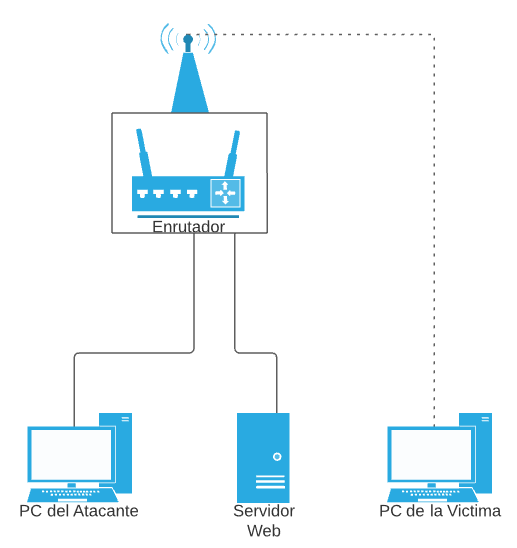
\includegraphics[width=9cm,height=9cm]{red.png}
       \end{center}
       \caption{Escenario montado}
    \end{figure}
 \end{center}

La idea principal de esta sección es demostrar que, encontrándose en una red interna
y con herramientas ya desarrolladas y libres, es posible realizar un ataque 
sin necesidad de conocer a fondo la implementación de la misma ni de tener mayores
privilegios.

El escenario consiste en crear una página web con un 
simple formulario donde se debe completar con usuario y contraseña, y un 
submit el cual envía esta información desde el cliente hasta el 
servidor web. El envío de este formulario contiene la información confidencial,
 por lo que en un escenario seguro ningún
intermediario podría obtener estos datos. Dado que este tráfico va a 
circular por HTTP, demostraremos como nos podemos hacer de las credenciales
ingresadas por el usuario.

\begin{center}
   \begin{figure}   
      \begin{center}
         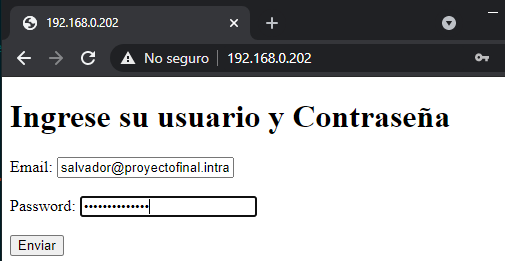
\includegraphics[width=10cm,height=6cm]{form.png}
      \end{center}
      \caption{Formulario montado}
   \end{figure}
\end{center}

Recordar que esto fue realizado en una red interna donde son todos equipos de nuestra propiedad.


\subsection{Preparando Ettercap para el ataque ARP Poisoning}

Lo primero que debemos hacer, en la lista de aplicaciones, es buscar el apartado 
\emph{Sniffing} y \emph{Spoofing}, ya que es allí donde encontraremos las herramientas necesarias
 para llevar a cabo este ataque. A continuación, abriremos Ettercap.

\begin{center}
    \begin{figure}   
       \begin{center}
          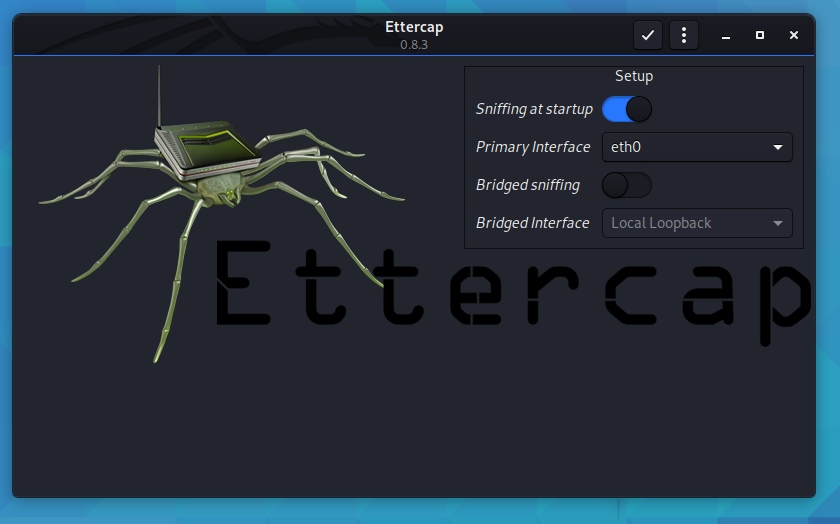
\includegraphics[width=9 cm,height=6cm]{ataque-2.png}
       \end{center}
       \caption{Ettercap}
    \end{figure}
 \end{center}

El siguiente paso es seleccionar la tarjeta de red con la que vamos a trabajar. Para 
ello, en el menú superior de Ettercap seleccionaremos Sniff $>$ Unified Sniffing y, 
cuando nos lo pregunte, seleccionaremos nuestra tarjeta de red (por ejemplo, en 
nuestro caso, eth0).

Luego se debe buscar todos los hosts conectados a nuestra red local. Para ello, 
seleccionaremos Hosts del menú de la parte superior y seleccionaremos la primera 
opción, Hosts List.

Allí deberían salirnos todos los hosts o dispositivos conectados a nuestra red. 
Sin embargo, en caso de que no salgan todos, podemos realizar una exploración 
completa de la red simplemente abriendo el menú Hosts y seleccionando la opción 
Scan for hosts. Tras unos segundos, la lista de antes se debería actualizar 
mostrando todos los dispositivos, con sus respectivas IPs y MACs, conectados 
a nuestra red.



\subsection{Nuestro Ettercap ya está listo. Ya podemos empezar con el ataque ARP Poisoning}

En caso de querer realizar un ataque dirigido contra un solo host, por ejemplo, 
suplantar la identidad de la puerta de enlace para monitorear las conexiones 
de la víctima, antes de empezar con el 
ataque debemos establecer los dos objetivos.

Para ello, debajo de la lista de hosts podemos ver tres botones, aunque nosotros 
prestaremos atención a los dos últimos:

    Target 1 – Seleccionamos la IP del dispositivo a monitorear, en este caso, 
    la computadora de la víctima, y pulsamos sobre dicho botón.

    Target 2 – Pulsamos la IP que queremos suplantar, en este caso, la de la 
    puerta de enlace y la del servidor web.

    \begin{center}
        \begin{figure}   
           \begin{center}
              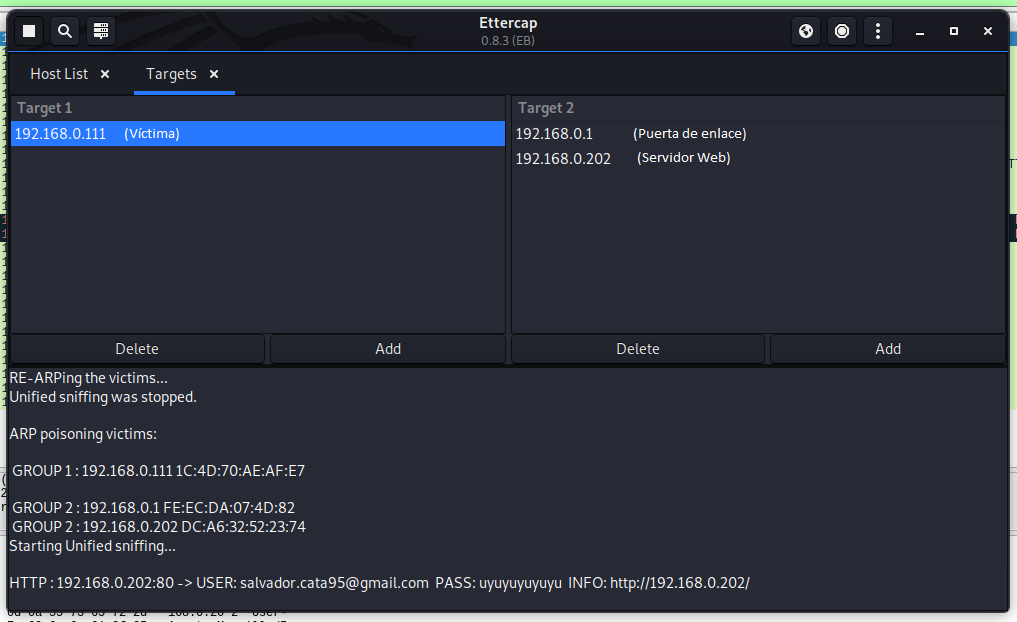
\includegraphics[width=17cm,height=9.5cm]{ataque-7-deta.png}
           \end{center}
           \caption{Ettercap}
        \end{figure}
     \end{center}

Todo listo. Ahora solo debemos elegir el menú MITM de la parte superior y, en él, 
escoger la opción ARP Poisoning. Nos aparecerá una pequeña ventana de configuración, 
en la cual debemos asegurarnos de marcar Sniff Remote Connections.
Pulsamos sobre Ok y el ataque dará lugar. Ahora ya podemos tener el control 
sobre el host que hayamos establecido como Target 1. Lo siguiente que debemos 
hacer es, ejecutar Wireshark para capturar todos los paquetes de 
red y analizarlos en busca de información interesante.

\begin{center}
   \begin{figure}   
      \begin{center}
         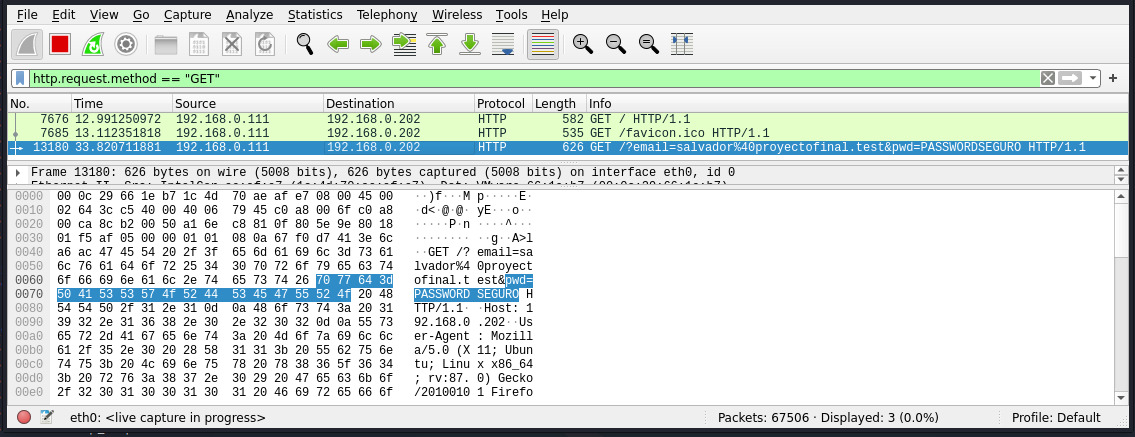
\includegraphics[width=17cm,height=7cm]{paquetes.png}
      \end{center}
      \caption{Paquetes capturados}
   \end{figure}
\end{center}

Como se puede ver, Wireshark nos permite filtrar el tráfico, y con el 
simple hecho de decirle que queremos mostrar los requerimientos GET
pudimos dar con el paquete que queríamos, en el request podemos ver
el usuario “salvador@proyectofinal.test” y la contraseña “PASSWORD SEGURO”


